\documentclass{beamer}


\mode<presentation>{
\usepackage{tikz}
\usetheme{JuanLesPins} 
\usepackage{amsmath}
\usepackage{array}
\usecolortheme{dolphin} 
}
\usepackage{graphicx} 
\usepackage{booktabs} 


\title[Project]{EE1390 P1} 
\title{EE1390 Project - 1}
\subtitle{Solving a Coordinate  Geometry Problem with Matrices}
\author{Raagini Vishnubotla EE17BTECH11050 \\
   Sai Manasa Pappu EE17BTECH11036} 
\date{IIT Hyderabad, Feb 2019}


\begin{document}


\begin{frame}
\titlepage 
\end{frame}


% Presentation slides begin
\begin{frame}{Index}
  \tableofcontents
\end{frame}

\section{Geometry Question}
\section{Matrix transformation of Question}
\section{Approach/Strategy}
\section{Solution}
\section{Figure of Solution}


\begin{frame}
\frametitle{Geometry Question}
\begin{block}{Question 52 in JEE Main 2015 Code D}
\bigbreak
The normal to the curve, $x^2 + 2xy - 3y^2 = 0$, at (1, 1) 
\bigbreak
(1) does not meet the curve again.\\
(2) meets the curve again in the second quadrant.\\
(3) meets the curve again in the third quadrant.\\
(4) meets the curve again in the fourth quadrant.
\bigbreak
\end{block}
\end{frame}


\begin{frame}
\frametitle{Matrix Transformation of Question}
\begin{block}{Rewriting in the form of matrices...}
Find the direction vectors, and normal vectors (as column vectors), to the pair of lines represented by the equation $x^2 + 2xy - 3y^2 = 0$. \\
If a normal is drawn at (1,1), find out in which quadrant it intersects the curve again, i.e.,\\
If M stores the normal vector of the normal at (1,1) as $M_1$, and the normal vector of the other line as $M_2$ as$M = \begin{pmatrix} M_1 & M_2 \end{pmatrix}$, and \\
$K = \begin{pmatrix} \begin{pmatrix} 1 \\ 1 \end{pmatrix}M1 & \begin{pmatrix}0\\0\end{pmatrix} M_1 \end{pmatrix}$. 
Find X such that \\
$K = X^T M \\
X^T = KM^{-1}$
\end{block}
\end{frame}


\begin{frame}
\frametitle{Approach/Strategy}
\begin{block}{Approach}
Given equation: $x^2 + 2xy - 3y^2 = 0$ \\
\\
The equation is in the form of a general second degree equation \\
$ax^2 + 2hxy + by^2 + 2gx + 2fy + c = 0$ \\
with g, f, c = 0. \\ 
\\
In such a case, the condition to be satisfied for the equation to represent a pair of straight lines is $h^2$ $\geq$ $ab$, which holds for the given equation. \\
Also, the above lines pass through the origin as (0,0) satisfies the equation. 
\end{block}
\end{frame}


\begin{frame}
\frametitle{}
\begin{block}{Strategy}
  \begin{itemize}
  \item
    Split the above combined equation into two individual lines.
  \item
    Find the line on which the given point (1,1) lies, say \textit{l1}.
  \item
    Using the direction vector of this line, find the normal vector.
  \item
    The line passing through (1,1) with direction vector as normal vector as computed above is our required new line.
    \begin{itemize}
    \item
      If this line is parallel to \textit{l2}, they do not intersect.
    \item
      Else, they intersect.
    \end{itemize}
  \end{itemize}
\end{block}
\end{frame}


\begin{frame}
\frametitle{Solution}
\\
Given combined line equation: x^2 + 2xy - 3y^2 = 0 \\
It can be rewritten as \[\frac{x^2}{y^2} + 2\frac{x}{y} - 3 = 0\] \\
which is in the form at^2 + bt + c = 0. \\
\bigbreak
It can be split into individual lines using the quadratic roots formula, \\
\[t = \frac{-b \pm \sqrt{b^2 - 4ac}}{2a} \] \\
\[\frac{x}{y} = \frac{-2 \pm \sqrt{(-2)^2 - 4\times(-3)}}{2} \]
\end{frame}


\begin{frame}
\frametitle{}
Therefore, we get the two following lines: \\
\[\frac{x}{y} = 1\]
\[\frac{x}{y} = -3\]\\
\bigbreak
Let M be a matrix that stores the direction vectors of the lines as \\
M = \begin{pmatrix} M_1 & M_2 \end{pmatrix}. Therefore, \\
\[M = \begin{pmatrix} 1 & -3 \\ 1 & 1 \end{pmatrix} \] \\
\bigbreak
Let N denote a matrix that stores the normal vectors of the lines as \\
N = \begin{pmatrix} N_1 & N_2 \end{pmatrix}. So,
\[N = \begin{pmatrix} 0 & -1 \\ 1 & 0 \end{pmatrix} 
\begin{pmatrix} 1 & -3 \\ 1 & 1 \end{pmatrix} 
= \begin{pmatrix} -1 & -1 \\ 1 & -3 \end{pmatrix}
\]
\end{frame}


\begin{frame}
\frametitle{}
The point P (1,1) lies on that line whose normal is $\perp^r$ to P-O = (1-0 , 1-0), since two lines intersect at the origin.\\
\bigbreak
$ P^TN = \begin{pmatrix}1 & 1\end{pmatrix} 
N = \begin{pmatrix} 0 & -4 \end{pmatrix}$ \\
Let the new line obtained at P by drawing a normal to the curve at that point, be \textit{l3}. \\
\bigbreak
$\textit{l3}: (x^T-
\begin{pmatrix} 1 & 1 \end{pmatrix} )$
$\begin{pmatrix} 1 \\ 1 \end{pmatrix} = 0$ 
or $x^T
\begin{pmatrix} 1 \\ 1 \end{pmatrix} = 2$ 
\bigbreak
$\textit{l2}: x^T
\begin{pmatrix} -1 \\ -3 \end{pmatrix}=0$
\bigbreak
Since \textit{l3} is not parallel to \textit{l2}, they have a point of intersection. \\
Let this point be x_o. 
\end{frame}


\begin{frame}
\frametitle{}
Since $x_o$ satisfies both the above equations, we have\\
\bigbreak

$x_{o}^T  
\begin{pmatrix} 1 & -1 \\ 1 & -3 \end{pmatrix} =
\begin{pmatrix} 2 & 0 \end{pmatrix} $
\bigbreak

$x_o^T = 
\begin{pmatrix} 2 & 0 \end{pmatrix} \times 
\begin{pmatrix} 1 & -1 \\ 1 & -3 \end{pmatrix}^{-1}$
\bigbreak

$x_{o}^T = 
\begin{pmatrix} 2 & 0 \end{pmatrix} 
\times -0.5 \times 
\begin{pmatrix} -3 & 1 \\ -1 & 1 \end{pmatrix} 
= -0.5 \times 
\begin{pmatrix} -6 & 2 \end{pmatrix} = 
\begin{pmatrix} 3 & -1 \end{pmatrix}$
\end{frame}


\begin{frame}
\frametitle{}
Therefore, the point of Intersection is
\bigbreak
$x_{o} = 
\begin{pmatrix} 3 & -1 \end{pmatrix}^T =
\begin{pmatrix} 3 \\ -1 \end{pmatrix}$
\bigbreak
which lies in the IV quadrant.
\bigbreak
Hence, the correct answer is - \\
(4) Meets the curve again in the fourth quadrant.
\end{frame}


\begin{frame}{Figure of Solution}
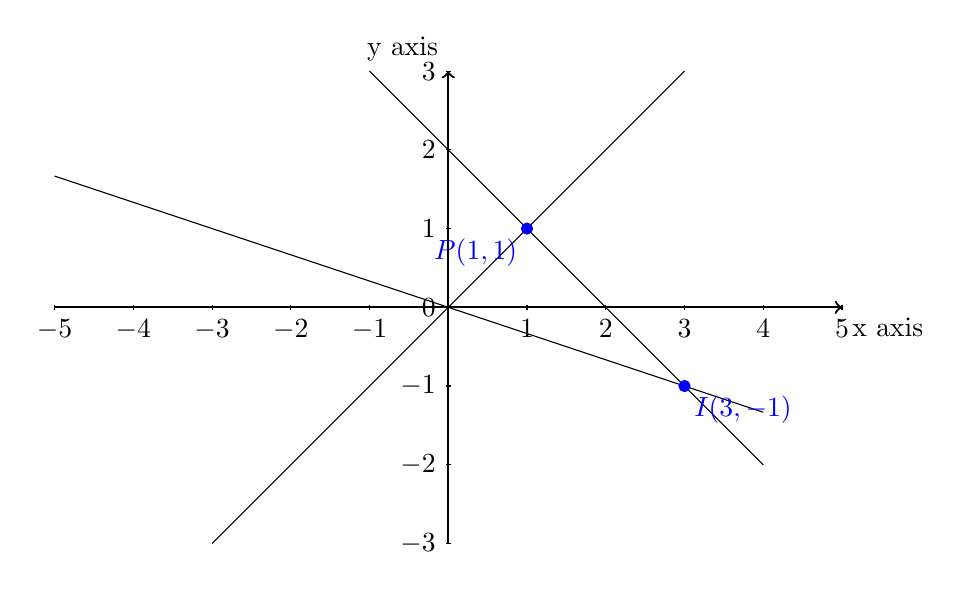
\begin{tikzpicture}
\begin{scope}
\draw[thick,->] (-5,0) -- (5,0) node[anchor=north west] {x axis};
\draw[thick,->] (0,-3) -- (0,3) node[anchor=south east] {y axis};
\foreach \x in {-5,-4,-3,-2,-1,1,2,3,4,5}
   \draw (\x cm,1pt) -- (\x cm,-1pt) node[anchor=north] {$\x$};
\foreach \y in {-3,-2,-1,0,1,2,3}
    \draw (1pt,\y cm) -- (-1pt,\y cm) node[anchor=east] {$\y$};
\draw (-3,-3) -- (3,3);
\draw (4,-4/3) -- (-5,5/3);
\draw (-1,3) -- (4,-2);
\filldraw[blue](1,1) circle (2pt) node[anchor=north east] {$P(1,1)$};
\filldraw[blue](3,-1) circle (2pt) node[anchor=north west] {$I(3,-1)$};
\end{scope}

\end{tikzpicture}
\end{frame}


\end{document}
